\documentclass[10pt]{article}

% Ћирилица
\usepackage[T2A]{fontenc}
\usepackage[utf8]{inputenc}
\usepackage[serbianc]{babel}

\usepackage[a4paper,top=1.5cm,bottom=1.5cm,left=1.8cm,right=1.8cm]{geometry}
\usepackage{amsmath}
\usepackage{multicol}
\usepackage{titlesec}
\titleformat*{\section}{\large\bfseries}
\titlespacing*{\section}{0pt}{6pt}{3pt}
\usepackage{enumitem}
\usepackage{tcolorbox}
\tcbuselibrary{breakable}
\usepackage[european]{circuitikz}
\usetikzlibrary{arrows.meta, babel}

\usepackage{diagbox}
\usepackage{colortbl} % (опционо, ако желиш сиву позадину заглавља као у књизи)

\pagestyle{empty}
\setlength{\columnsep}{0.8cm}
\setlength{\parindent}{0pt}
\setlength{\parskip}{3pt}

% Оквир за кључне податке
\newtcolorbox{kljucno}{colback=blue!4, colframe=blue!45!black,
    boxrule=0.5pt, arc=1.5pt, left=6pt, right=6pt, top=3pt, bottom=3pt}

% Решени пример
\newtcolorbox[auto counter]{primer}{
    colback=white, colframe=black!55, colbacktitle=black!55, coltitle=white,
    fonttitle=\bfseries\small, title={Пример~\thetcbcounter},
    boxrule=0.5pt, arc=1.5pt, left=5pt, right=5pt, top=2pt, bottom=2pt,
    before skip=5pt, after skip=5pt}

% Задатак за вежбу (решење се даје само као резултат)
\newtcolorbox[auto counter]{zadatak}{
    colback=green!3, colframe=green!40!black, colbacktitle=green!40!black, coltitle=white,
    fonttitle=\bfseries\small, title={Задатак~\thetcbcounter},
    boxrule=0.5pt, arc=1.5pt, left=5pt, right=5pt, top=2pt, bottom=2pt,
    before skip=5pt, after skip=5pt}

\begin{document}

\begin{center}
    {\LARGE\bfseries Лабораторијске вежбе из основа електротехнике} \\
    {\Large Мерење физичких појава.} \\
\end{center}
\vspace{6pt}

\begin{multicols}{2}

\section{Мерне величине и јединице}



\textbf{Основне} мерне величине и њихове основне јединице су: 

\begin{itemize}
  \item Дужина [m] - \textit{метар}
  \item Маса [kg] - \textit{килограм}
  \item Време [s] - \textit{секунд}
  \item Електрична струја [A] - \textit{Ампер}
  \item Температура [K] - \textit{Келвин}
  \item Јачина светлости [cd] - \textit{кандел}
  \item Количина материје [mol] - \textit{мол}
\end{itemize}

Ове величине се другачије називају \textbf{SI} мерне величине, назване по институцији одакле су добиле име, Међународни 
систем јединица \textit{(енг. International System of Units)}. Јединице које не приадају \textit{SI} а користе се
често називају се \textbf{изведене величине} и \textbf{изведене јединице}. Основна одлика оваквих јединица је да се њихова квантитативна вредност
може изразити преко основних јединица

%==================================================================
\section{Префикси и степени броја 10}
%==================================================================

Како би се лакше представљале велике и мале квантитативне вредности неких
величина у свакодневну анализу и мерење убачени су такозвани \textbf{префикси}.
Префикси представљају неки степен броја 10, на пример кило \textit{к} износи $1000 = 10^3$
пута веће.

\end{multicols}

\begin{table}[htbp]
  \centering
  % Лева табела: Веће јединице (са 1 на дну)
  \begin{minipage}[t]{0.40\textwidth}
    \centering
    \caption{Веће јединице (умношци)}
    \begin{tabular}{|c|l|c|}
      \hline
      \textbf{Ознака} & \textbf{Назив} & \textbf{Степен} \\ \hline
      Y & јота & $10^{12}$    \\ \hline
      Z & зета & $10^{12}$    \\ \hline
      E & екса & $10^{12}$    \\ \hline
      P & пета & $10^{12}$    \\ \hline
      T  & тера & $10^{12}$    \\ \hline
      G  & гига & $10^{9}$     \\ \hline
      M  & мега & $10^{6}$     \\ \hline
      k  & кило & $10^{3}$     \\ \hline
      h   & хекто & $10^{2} = 100$     \\ \hline
      da & дека & $10^{1} = 10$     \\ \hline
      -- & --   & $10^{0} = 1$ \\ \hline
      \multicolumn{3}{c}{} \\ % Празан невидљиви ред ради поравнања висине
    \end{tabular}
  \end{minipage}
 \hspace{0.01cm}
  % Десна табела: Мање јединице (са 1 на врху)
  \begin{minipage}[t]{0.40\textwidth}
    \centering
    \caption{Мање јединице (делови)}
    \begin{tabular}{|c|l|c|}
      \hline
      \textbf{Ознака} & \textbf{Назив} & \textbf{Степен} \\ \hline
      --    & --    & $10^{0} = 1$ \\ \hline
      d     & деци  & $10^{-1} = 0.1$    \\ \hline
      c     & центи & $10^{-2} = 0.01$    \\ \hline
      m     & мили  & $10^{-3}$    \\ \hline
      $\mu$ & микро & $10^{-6}$    \\ \hline
      n     & нано  & $10^{-9}$    \\ \hline
      p     & пико  & $10^{-12}$   \\ \hline
      f     & фемто & $10^{-15}$   \\ \hline
      a     & ато   & $10^{-18}$    \\ \hline
      z     & зепто & $10^{-21}$    \\ \hline
      y     & јокто & $10^{-24}$    \\ \hline
    \end{tabular}
  \end{minipage}
\end{table}

\section{Пример мерења}

Нека је за мерење срчаног пулса (енг. \textit{heartbeat}) помоћу електрокардиографа 
(ЕКГ) потребно израчунати растојање између два R зупца (трајање RR интервала). 
R зубац представља локални максимум периодичног ЕКГ сигнала. На слици 1, дат 
је пример ЕКГ сигнала: на екрану осцилоскопа приказане су три периоде ЕКГ 
сигнала и означена су одговарајућа три R зупца.

\begin{figure}[htbp]
  \centering
  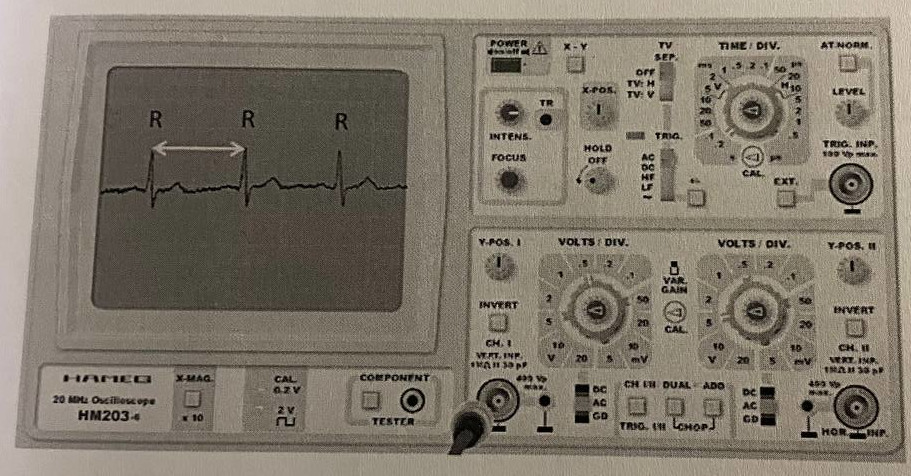
\includegraphics[width=0.6\linewidth]{ekg_signal.jpg}
  \caption{ЕКГ сигнал приказан на екрану осцилоскопа.}
\end{figure}

Мерењем временског интервала $T_{RR}^1$ (растојање између два R зупца означено на 
слици 1), добија се да је $T_{RR}^1 = 1\text{ s}$. Међутим, на слици 1 приказан је и 
други RR интервал, а његова вредност је $T_{RR}^2 = 0.9\text{ s}$.
Нека је RR интервал мерен 10 пута на 5 различитих испитаника $(ID1–5)$ и нека 
су резултати приказани у табели:

\begin{table*}[htbp]
  \centering
  \caption{Резултати мерења за $n = 10$ поновљених мерења RR интервала за пет испитаника (ID1–5).}
  \begin{tabular}{|l|c|c|c|c|c|c|c|c|c|c|}
    \hline
    \diagbox{$T_{RR}^n$ [s]}{$N$} & \textbf{1} & \textbf{2} & \textbf{3} & \textbf{4} & \textbf{5} & \textbf{6} & \textbf{7} & \textbf{8} & \textbf{9} & \textbf{10} \\ \hline
    \textbf{ID1} & 1.0 & 0.9 & 0.9 & 0.9 & 1   & 0.9 & 0.9 & 0.9 & 0.9 & 1.0 \\ \hline
    \textbf{ID2} & 1.0 & 1.0 & 1.0 & 0.6 & 1.0 & 1.0 & 1.0 & 1.0 & 0.7 & 1.0 \\ \hline
    \textbf{ID3} & 0.8 & 0.8 & 0.8 & 0.8 & 0.8 & 0.8 & 0.8 & 0.9 & 0.8 & 0.8 \\ \hline
    \textbf{ID4} & 0.6 & 0.7 & 0.8 & 1.0 & 1.0 & 1.0 & 0.7 & 0.8 & 0.9 & 0.7 \\ \hline
    \textbf{ID5} & 0.6 & 0.6 & 0.6 & 1.0 & 1.0 & 1.0 & 1.0 & 1.0 & 0.6 & 0.6 \\ \hline
  \end{tabular}
\end{table*}

Из добијених резултата, може се закључити да квантитативне вредности поновљених 
мерења нису исте. На пример, за испитаника ID1 нека мерења указују на то да је 
дужина RR интервала $0.9\text{ s}$, а друга мерења на то да је дужина RR интервала 
$1\text{ s}$. Разлог томе може бити велики број фактора који утичу на мерење (однос 
сигнал / шум, померање електрода, нестабилан \textit{offset} потенцијал електрода, 
метода детекције R интервала и друге), али и физиолошких фактора које није могуће одредити 
детерминистички тј. једнозначно.

\section{Средња вредност и мерна несигурност}

Како бисмо једноставније представили резултате наших мерења, користимо
\textbf{средњу вредност} и \textbf{мерну несигурност} измерених резултата.

\begin{figure}[htbp]
  \centering
  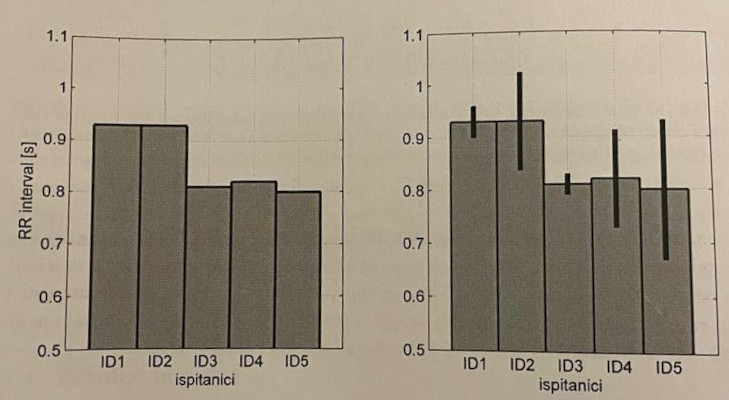
\includegraphics[width=0.6\linewidth]{merenja.jpg}
  \caption{Графички приказ резултата мерења.}
\end{figure}

Са леве слике, графички су приказане \textbf{средњу вредности} временских интервала $T_{RR}$
по човеку $(ID)$. Наизглед може деловати као да су $(ID1)$ и $(ID2)$ иста мерења. Разлог
томе је информација коју смо изоставили овим графичким приказом, колико се разликују информације. 
Детаљнији увид добијамо
када уведемо \textbf{мерну несигурност} која се репрезентује као црне линије на десном графику.
На пример, видимо да је $(ID1)$ у опсегу [0.9 - 1.0] а $(ID2)$ [0.7 - 1.0]. Мерна несигурност 
нам даје информацију о расподели резултата мерења од средње вредности.

\begin{kljucno}
Из мерења која имамо, извлачимо информације о средњој вредности и мерној несигурности, 
и финалан резултат можемо онда представити нумерички по следећем исказу: 

\begin{equation}
  x = \tilde{x} \pm u
\end{equation}

У горе наведеном изразу, $x$ представља финалан резултат, $\tilde{x}$ средњу вредност а $u$, мерну несигурност.

\end{kljucno}

\end{document}